%!TEX root = ../main.tex

% datasets table..
\begin{table*}[b]
 {
  \begin{tabular}[c]{llrrrc|rrrr} \toprule
   Network &  Description & $|V|$           & $|E|$        & $T$        & $A$, $|A|$  &  \texttt{LN} $(\mu, \sigma)$ & \texttt{DPL} $\alpha$       &  Avg. ${\texttt{LCC}}$  & \texttt{AA} $r$           \\ \midrule
   \texttt{USSC}~\cite{fowler2008authority}  & U.S. Supreme Court cases         & 30,288     & 216,738      & 1754-2002  & -   & (1.19, 1.18) & 2.32     & 0.12    & -     \\
   \texttt{HEP-PH}~\cite{gehrke2003overview} & ArXiv Physics manuscripts     & 34,546     & 421,533      & 1992-2002  & -  &   (1.32, 1.41) & 1.67     & 0.12    & -                 \\
   \texttt{Semantic}~\cite{ammar}&   Academic Search Engine  & 7,706,506  & 59,079,055   & 1991-2016  & -   &   (1.78, 0.96)  & 1.58     & 0.06    & -             \\   \midrule
   \texttt{ACL}~\cite{acldata}    & NLP papers      & 18,665     & 115,311      & 1965-2016  & \textsc{venue}, 50  &   (1.93, 1.38)  & 1.43     & 0.07    & 0.07  \\
   \texttt{APS}~\cite{aps}     & Physics journals     & 577,046    & 6,967,873    & 1893-2015  & \textsc{journal}, 13 &   (1.62, 1.20)  & 1.26     & 0.11    & 0.44 \\
   \texttt{Patents}~\cite{leskovec2005graphs}   & U.S. NBER patents    & 3,923,922  & 16,522,438   & 1975-1999  & \textsc{category}, 6 &   (1.10, 1.01)   & 1.94     & 0.04    & 0.72 \\
   % \texttt{PYPI}         & 25,169     & 71,371       & 2002-2018  & \textsc{category} & 9  \\
  \bottomrule
  \end{tabular}
  \vspace{1mm}
  \caption{Summary statistics \& global properties of six network datasets: $|V|$ nodes join the networks and form edges $|E|$ over
  time period $T$. In attributed networks, each node has a categorical attribute value that belongs to set $A$ of size $|A|$.
  The networks exhibit lognormal (\texttt{LN}) in-degree distribution with mean $\mu$ and standard deviation $\sigma$,
  high average local clustering (${\texttt{LCC}}$) \& attribute assortativity (\texttt{AA}) coefficient and
  densify over time with power law (\texttt{DPL}) exponent $\alpha$.}
  \label{table:datasets}
  \label{table:netstats}
 }
\end{table*}


\section{Introduction}
\label{sec:Introduction}

\begin{figure}
	\centering
	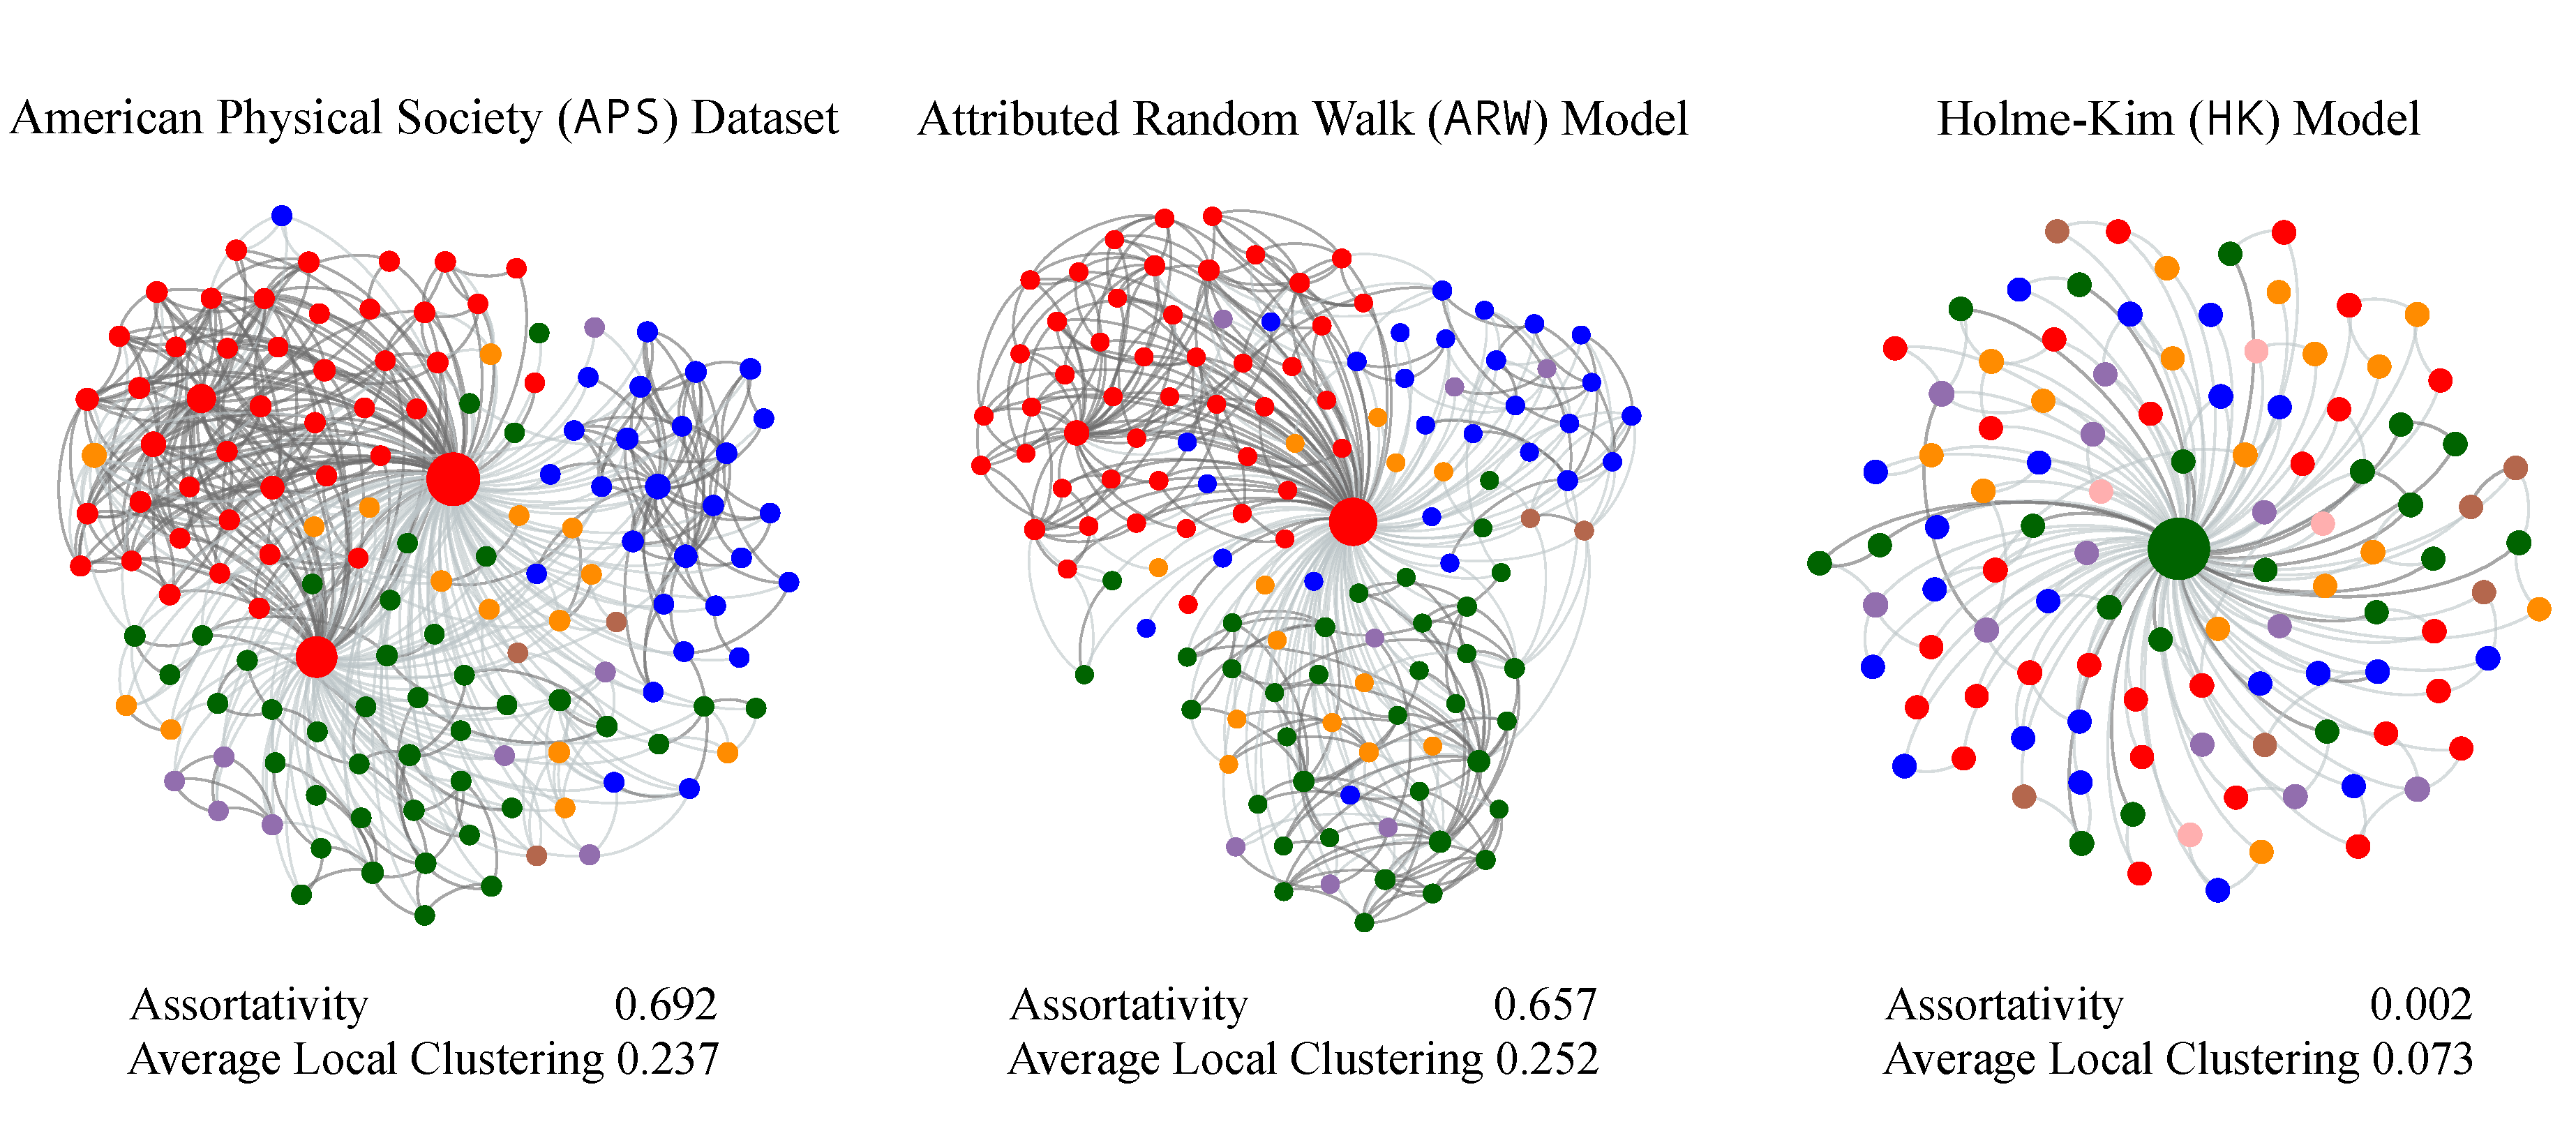
\includegraphics[width=\columnwidth]{introduction_plot}
    \caption{We contrast our proposed model, Attributed Random Walk (\texttt{ARW}), with a non-attributed growth model~\cite{holme2002growing} to underscore the importance of using attributes for network growth.}
	\label{fig:intro_plot}
  \vspace{-20pt}
\end{figure}



% what is the problem?

We present a network growth model that explains how distinct
structural properties of attributed networks can emerge from a local edge
formation process. In real-world networks, individuals form edges
with limited information and partial network access.
Moreover, phenomena such as triadic closure and homophily
simultaneously influence individuals' decisions to form connections.
Over time, these decisions cumulatively shape real-world networks to exhibit
rich structural properties: heavy-tailed in-degree distribution, skewed
local clustering and diverse attribute mixing patterns. However, we lack an
understanding of local, resource-constrained mechanisms that incorporate
sociological factors to jointly explain the emergence of multiple structural properties.
Additionally, accurate network growth models are useful for synthesizing networks and extrapolating existing real-world networks.


% why is it important?

Well-known models of network growth tend to make unrealistic assumptions about how
individuals form edges. Consider a simple stylized example: the process of
finding a set of papers to cite when writing an article. In preferential
attachment \cite{barabasi1999emergence} or fitness
\cite{bianconi2001bose,caldarelli2002scale,wang2013quantifying} based models, a
node making $m$ citations would pick papers from the \textit{entire} network in
proportion to their in-degree or fitness respectively. This process assumes that
individuals possess {complete} knowledge of in-degree or fitness of every node
in the network. An equivalent formulation---vertex copying
\cite{kumar2000stochastic}---induces preferential attachment: for every
citation, a node would pick a paper uniformly at random from \textit{all}
papers, and either cite it or copy its citations. Notice that vertex copying assumes individuals have complete access to the network and forms each
edge independently. Although these models explain the emergence of power law
degree distributions, they are unrealistic: preferential attachment and vertex
copying require global node-level knowledge or complete network access respectively.
Additionally, they do not account for the role of assortative mixing ~\cite{newman2002assortative} via nodal attributes (e.g., venue of paper, political interests of Facebook users) in network formation.

Recent papers account for resource constraints
\cite{mossa2002truncation,zeng2005construction,wang2009local} and nodal
attributes \cite{de2013scale,gong2012evolution}. However, the former disregard
attributes and the latter do not provide a realistic representation of edge
formation under constraints. Furthermore, both sets of models do not
jointly preserve multiple structural properties.

We aim to develop a growth model that accounts for resource constraints and sociological phenomena
influencing edge formation in addition to preserving global network structure.
We make three key contributions.
First, we propose a simple and accurate model of attributed network growth.
Second, our model is based on local processes to form edges, without recourse to global network information.
Third, our model unifies multiple sociological phenomena---bounded rationality; structural constraints; triadic closure; attribute homophily; preferential attachment---to jointly  model global network structure and attribute mixing patterns.


The proposed model---Attributed Random Walk (\texttt{ARW})---jointly explains
the emergence of in-degree distribution, local clustering, clustering-degree
relationship and attribute mixing patterns through a resource constrained
mechanism based on random walks (see~\Cref{fig:intro_plot}). In particular,
the model relies entirely on local information to grow the network, without
access to information of all nodes. In \texttt{ARW}, incoming nodes select a
seed node based on attribute similarity and initiate a biased random walk: at
each step of the walk, the incoming node either jumps back to its seed or
chooses an outgoing link or incoming link to visit another node; it links to
each visited node with some probability and halts after it has exhausted its
budget to form connections.
Our experiments on six large-scale network datasets indicate that the proposed growth model outperforms
eight state-of-the-art network growth models by a
statistically significant margin of 2.5--$10\times$.


The rest of the paper is organized as follows.
We begin by defining the problem statement in~\Cref{sec:Problem Statement}.
In~\Cref{sec:Analysis}, we outline six network datasets, describe key structural
properties of real-world networks and discuss insights from sociological studies.
Then, in~\Cref{sec:Proposed Model}, we describe the network growth model. Then, We
present experiments in ~\Cref{sec:Experiments}, discuss related work in ~\Cref{sec:Related Work} and conclude in~\Cref{sec:Conclusion}.
